%%=================--------------------------------3.Giai thuat de xuat---------------------------========================
Chương \ref{Chap_mfeaGiaiCayPhanCum} sẽ đề xuất một giải thuật tiến hóa đa nhân tố CluMFEA đa nhiệm giải đồng thời bài toán CluMRCT và bài toán CSPT. Giải thuật CluMFEA đề xuất gồm có hai tác vụ, một tác vụ CluMRCT và một tác vụ CSPT. Sơ đồ của giải thuật CluMFEA này giống với giải thuật MFEA cơ bản như đã trình bày ở mục 1.2.4. Nội dung đề xuất mới bao gồm đề xuất về biểu diễn cá thể, khởi tạo quần thể, các toán tử lai ghép, đột biến cho CluMFEA giải hai bài toán cụ thể là CluMRCT và CSPT.

Ngoài ra, đồ án cũng đề xuất một giải thuật di truyền CluGA giải hai bài toán CluMRCT và CSPT. Vì là giải thuật đơn nhiệm nên CluGA chỉ có thể giải lần lượt từng bài trong hai bài toán CluMRCT và CSPT. Sơ đồ của giải thuật CluGA đề xuất giống với sơ đồ giải thuật di truyền đã nêu ở mục 1.1 của chương 1. Nội dung đề xuất mới bao gồm cách biểu diễn cá thể và các toán tử khởi tạo, lai ghép, đột biến. Các đề xuất này giống với các đề xuất về các toán tử tương ứng cho CluMFEA.

Phần sau trình bày lần lượt các nội dung đề xuất.



%%=================--------------------------------1.Biểu diễn cá thể---------------------------========================
\section{Biểu diễn cá thể} \label{chap_mfeaProposed:sec:bieudiencathe}
Biểu diễn cá thể (hay mã hóa lời giải) đóng vai trò quan trọng trong các giải thuật tiến hóa, bởi nó ảnh hưởng trực tiếp tới việc lựa chọn và xây dựng các toán tử tiến hóa. Do đó, biểu diễn cá thể cũng ảnh hưởng lớn tới hiệu quả của giải thuật CluMFEA và CluGA được đề xuất. Có rất nhiều cách để biểu diễn cá thể là cây khung như sử dụng mã Dandelion~\cite{perfecto_dandelion_encoded_2016}, mã Blob~\cite{julstrom2005blob},.. Tuy nhiên, nhiều nghiên cứu đã chỉ ra rằng mã hóa cây khung sử dụng tập cạnh là một trong các mã hóa hiệu quả nhất trong các bài toán tìm cây khung~\cite{julstrom_initialization_2002, raidl_edge_2003, rothlauf_representations_2008}. Vì vậy, trong đồ án này, mã hóa tập cạnh được sử dụng để biểu diễn lời giải của hai bài toán CluMRCT và CluSTP.


\renewcommand{\scalefigure}{0.5}
\begin{figure}[htbp]
	\centering		
	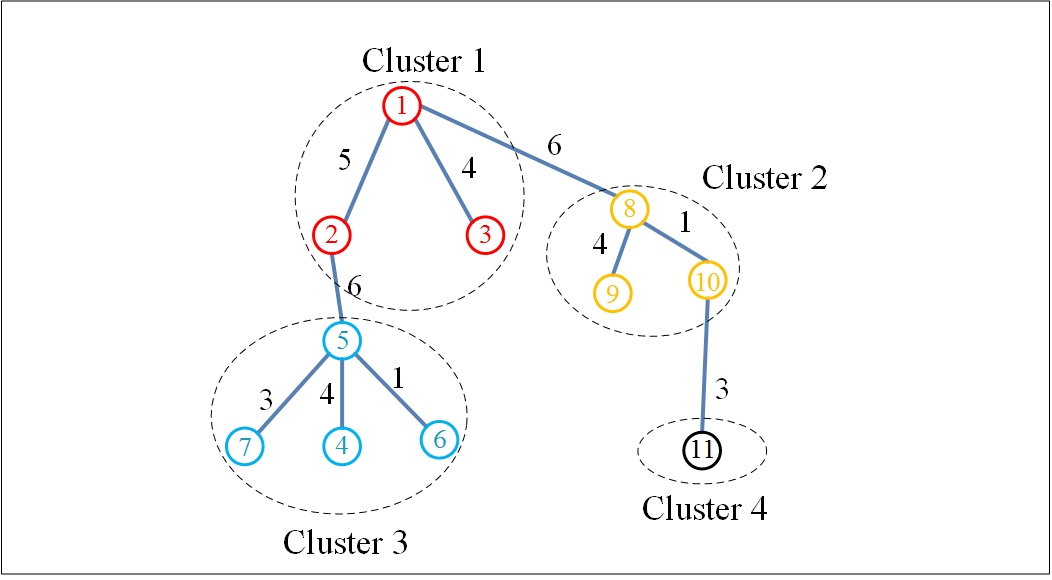
\includegraphics[scale=\scalefigure]{Pictures/Ind_representation/Ind_Representation.png}
	\centering
	\caption{Lời giải hợp lệ của bài toán CluMRCT và bài toán CSPT}
	\label{fig:ind_representation}
\end{figure}

Giả sử đồ thị trong hình~\ref{fig:ind_representation} là một lời giải hợp lệ của bài toán \gls{clumrct} và bài toán \gls{cstp}. Khi đó mã hóa tập cạnh tương ứng với lời giải này là \{(1,2); (1,3); (1,8); (2,5); (4,5); (5,7); (5,6); (8,9); (8,10); (10,11)\}.


%%=======--------------------------------2.	Khởi tạo quần thể---------------------------======
\section{Khởi tạo quần thể} \label{chap_mfeaProposed:sec:khoitaoquanthe}
Lời giải hợp lệ của bài toán \gls{cstp} và \gls{clumrct} là một cây khung T và các đồ thị cảm sinh của T trên mỗi cụm cũng là cây khung. Do đó, đồ án đề xuất một phương pháp khởi tạo ngẫu nhiên các cá thể luôn thỏa mãn các điều kiện ràng buộc của hai bài toán.

Các bước của giải thuật khởi tạo quần thể được trình bày trong thuật toán \ref{alg:DeXuatKhoiTaoCaThe}.
\begin{algorithm}[htb]
		\KwIn{Đồ thị $G=(V, E, w)$ và phân hoạch $R = \{R_1, R_2, R_3,\ldots,R_k\}$ của $V$}
		\KwOut{Một cây khung phân cụm $T_r=(V_r,E_r)$ của $G$}
		\BlankLine
	\Begin
	{	
		$V_r \leftarrow V$\;
		$G' \leftarrow$ H-Graph của đồ thị $G$\;
		$T' \leftarrow$ PrimRST($G'$) \Comment{Tạo cây khung ngẫu nhiên cho đồ thị H-Graph}\;
		\ForEach{cụm i-th}
		{
			$T_i \leftarrow$ PrimRST($G[R_i]$) \Comment{Tạo cây khung ngẫu nhiên cho cụm i}\;
		}
		$E_r \leftarrow \left( \cup_{i=1}^{k} E(T_i) \right)\cup E(T')$ \Comment{Hợp tập cạnh của cây khung của H-Graph và các cụm}\;
	}
	\caption{Khởi tạo một cá thể ngẫu nhiên}
	\label{alg:DeXuatKhoiTaoCaThe}
\end{algorithm}

%%=================--------------------------------3.Toán tử tiến hóa---------------------------========================
\section{Toán tử tiến hóa} \label{chap_mfeaProposed:sec:ToanTuTienHoa}
Toán tử lai ghép và đột biến được đề xuất luôn tạo ra cá thể hợp lệ cho cả hai bài toán \gls{clumrct} và bài toán \gls{cstp}. Chi tiết về các toán tử tiến hóa được trình bày dưới đây.

\subsection{Toán tử lai ghép} \label{chap_coso:sec_mfea:subsec:toantulaighep}
Trong toán tử lai ghép được đề xuất, các cạnh trên cá thể con đều được kế thừa từ các cạnh của một trong hai cá thể cha mẹ. Những cạnh xuất hiện ở cả 2 cá thể cha và cá thể mẹ sẽ chắc chắc được kế thừa ở cá  thể con. Điều này giúp đảm bảo việc lưu giữ các đặc điểm di truyền tốt cho thế hệ sau.

Các bước của toán tử lai ghép được trình bày trong thuật toán \ref{alg:laighepmoi}.
\begin{algorithm}[htb]
	\KwIn{Đồ thị $G=(V, E, w)$ và phân hoạch $R = \{R_1, R_2, \ldots,R_k\}$ của $V$; 
	\qquad \quad Cá thể cha mẹ: $T_{m}=\left(V,E_{m}\right), m = 1,2$.}
	\KwOut{Cá thể con $T_c = (V_c, E_c)$}
	\BlankLine
	\Begin
	{	
		$V_c \leftarrow V$\;
		\ForEach{cụm i-th}
		{
			$E_i \leftarrow E(T_1[R_i]) \cup E(T_2[R_i])$ \Comment{Hợp tập cạnh của cá thể cha mẹ của cụm i}\;
			$T_i \leftarrow$ PrimRST($(R_i, E_i$)) \Comment{Tạo cây khung ngẫu nhiên cho cụm i}\;
		}
		$T'_m \leftarrow$ H-Graph của đồ thị $T_m, m = 1,2$\;
		$T' \leftarrow$ PrimRST($T'_1 \cup T'_2$) \Comment{Tạo cây khung ngẫu nhiên cho đồ thị H-Graph}\;
		
		$E_c \leftarrow \left( \cup_{i=1}^{k} E(T_i) \right)\cup E(T')$ \Comment{Hợp tập cạnh của cây khung của H-Graph và các cụm}\;
	}
	\caption{Toán tử lai ghép mới}
	\label{alg:laighepmoi}
\end{algorithm}

\renewcommand{\scalefigure}{0.2}
\begin{figure}[tb]
	\centering	
	\setlength\tabcolsep{0 pt}
	\begin{tabular}{ccc}
		\renewcommand{\scalefigure}{0.203}
		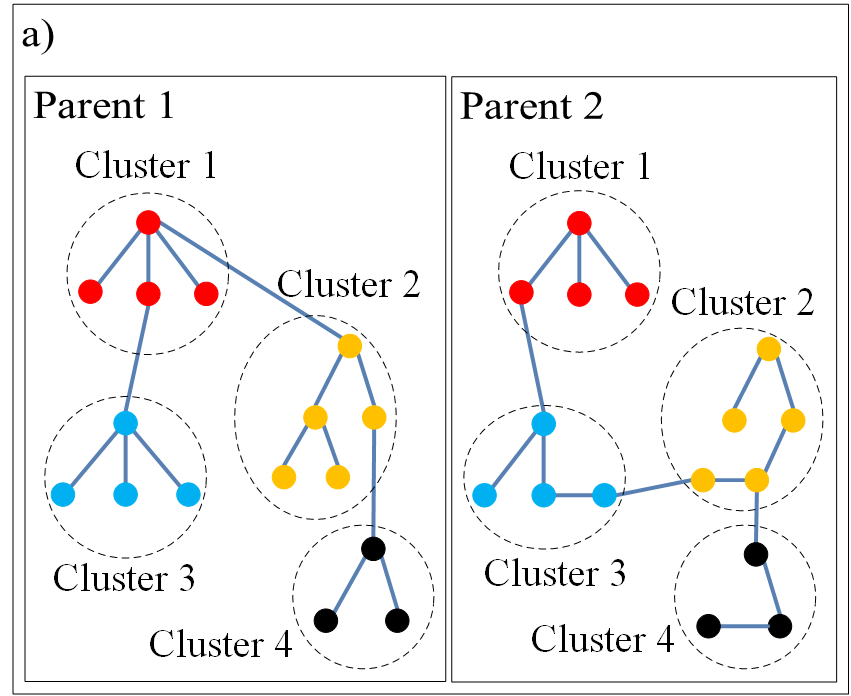
\includegraphics[scale=\scalefigure]{Pictures/Crossover/Crossover_New_a.png} &
		\renewcommand{\scalefigure}{0.20} 	
		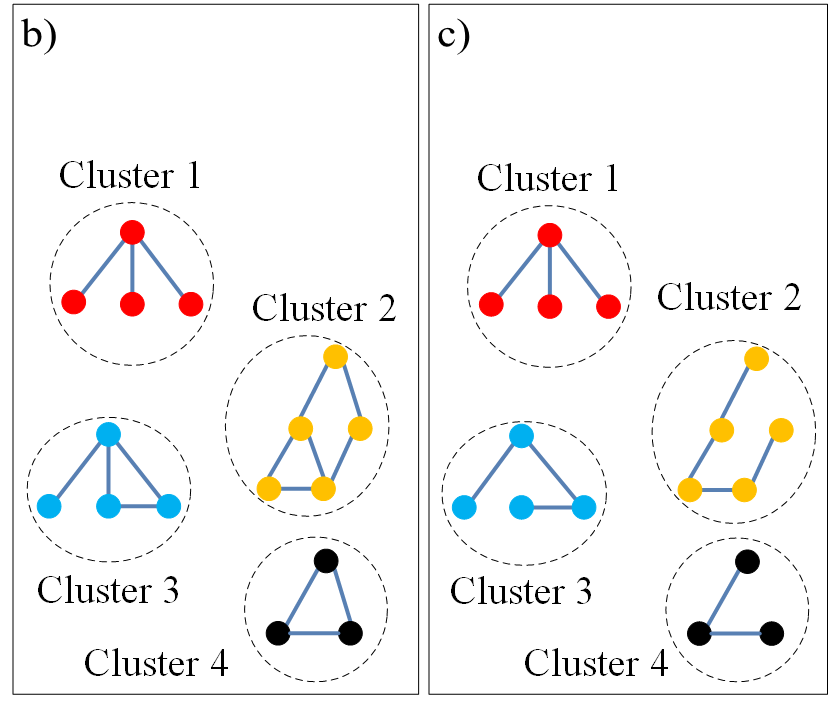
\includegraphics[scale=\scalefigure]{Pictures/Crossover/Crossover_New_b_c.png} &  
		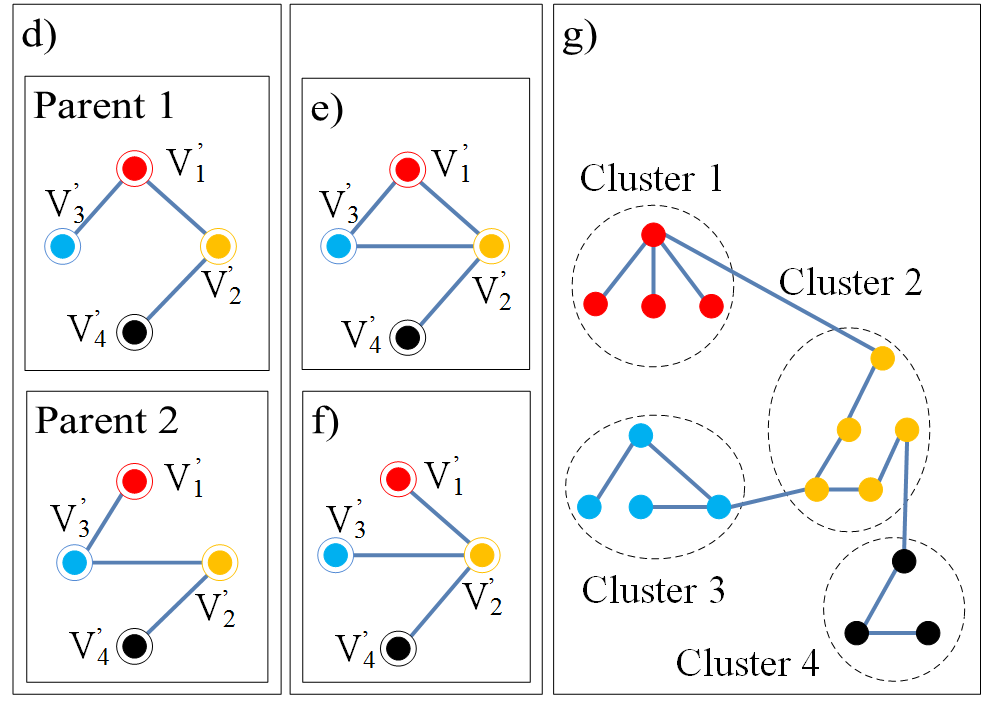
\includegraphics[scale=\scalefigure]{Pictures/Crossover/Crossover_New_d_e_f_g.png}\\
	\end{tabular}
	\centering
	\caption{Các bước lai ghép trong giải thuật MFEA đề xuất}
	\label{fig:Steps_of_novel_crossover_operator}
\end{figure}

Hình~\ref{fig:Steps_of_novel_crossover_operator} mô phỏng các bước của toán tử lai ghép trên. Trong đó,  Hình~\ref{fig:Steps_of_novel_crossover_operator}.a biểu diễn cá thể cha và cá thể mẹ trước khi được lai ghép. Đồ thị con của mỗi cluster sau khi hợp các cạnh của 2 cá thể cha mẹ được minh họa trong hình~\ref{fig:Steps_of_novel_crossover_operator}.b. Hình \ref{fig:Steps_of_novel_crossover_operator}.c minh họa các cây khung được tạo từ các đồ thị trong hình~\ref{fig:Steps_of_novel_crossover_operator}.b. sau khi áp dụng thuật toán PrimRST. Hình~\ref{fig:Steps_of_novel_crossover_operator}.d minh họa các H-Graph tương với các cá thể cha mẹ. Hình~\ref{fig:Steps_of_novel_crossover_operator}.e minh họa đồ thị nhận được sau khi hợp các H-Graph. Hình~\ref{fig:Steps_of_novel_crossover_operator}.f minh họa cây khung nhận được từ đồ thị trong Hình~\ref{fig:Steps_of_novel_crossover_operator}.e. sau khi áp dụng thuật toán PrimRST. Cá thể con được tao thành từ 2 cá thể cha mẹ được minh họa trong Hình~\ref{fig:Steps_of_novel_crossover_operator}.g.


\subsection{Toán tử đột biến} \label{chap_coso:sec_mfea:subsec:toantudotbien}
Ý tưởng chính của toán tử đột biến được tạo là tạo ra chu trình trên cá thể cha sau đó xóa bỏ cạnh trong chú trình đó để tạo thành cá thể mới hợp lệ.

Các bước của toán tử đột biến được trình bày trong thuật toán \ref{alg:dotbienmoi}.
\begin{algorithm}[htbp]
%	\SetAlgorithmName{MegaAlgorithm}{} %last arg is the title of listing table
%	\floatname{algorithm}{MegaAlgorithm}
	\KwIn{Cây khung $T_c$ của đồ thị G}
	\KwOut{Một cây khung con T}
	\BlankLine
	\Begin
	{	
		$R_i \leftarrow$ Chọn một cụm ngẫu nhiên của G\;
		$e \leftarrow$ Chọn cạnh ngẫu nhiên thuộc tập E($G[R_i]$) $\backslash$ E($T_c$)\;
		Thêm $e$ vào $T_c$ để tạo thành một chu trình $C$ trên $T_c$\;
		Xóa ngẫu nhiên cạnh $e' \in C$ thỏa mãn $e \neq e'$ \;
	}
	\caption{Toán tử Đột biến}
	\label{alg:dotbienmoi}
\end{algorithm}

Hình~\ref{fig:Illustation_of_new_mutation_operator} mô phỏng các bước trong thủ tục đột biến được đề xuất. Hình~\ref{fig:Illustation_of_new_mutation_operator}.a là cây khung $T_c$ trước khi bị đột biến. Hình~\ref{fig:Illustation_of_new_mutation_operator}.b minh họa đồ thị sau khi cụm thứ 3 (nền màu vàng) được chọn ngẫu nhiên. Hình~\ref{fig:Illustation_of_new_mutation_operator}.c minh họa đồ thị sau khi cạnh được thêm vào (cạnh nét đậm mầu đỏ) cụm thứ 3 để tạo thành chu trình. Hình~\ref{fig:Illustation_of_new_mutation_operator}.d minh họa đồ thị là kết quả của phép đột biến  sau khi một cạnh ngẫu nhiên khác cạnh vừa được thêm vào được loại bỏ khỏi $T_c$.

\renewcommand{\scalefigure}{0.26}
\begin{figure}[htb]
	\centering	
	\setlength\tabcolsep{0 pt}
	\begin{tabular}{cc}
		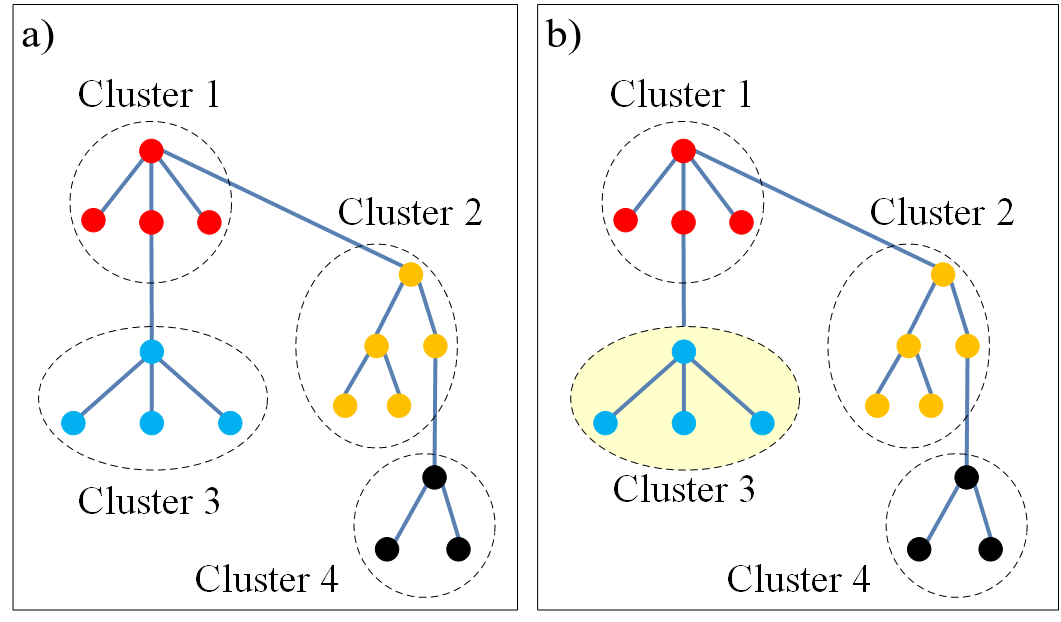
\includegraphics[scale=\scalefigure]{Pictures/Mutation/Mutation_a_b.png} & 	
		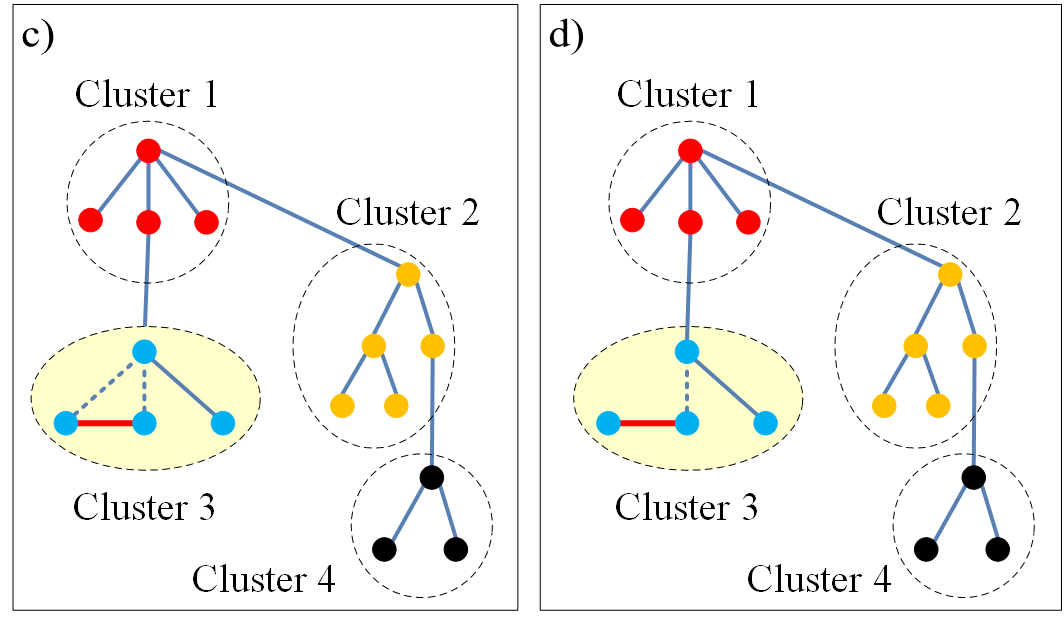
\includegraphics[scale=\scalefigure]{Pictures/Mutation/Mutation_c_d.png} \\
	\end{tabular}
	\centering
	\caption{Ví dụ minh họa toán tử đột biến mới}
	\label{fig:Illustation_of_new_mutation_operator}
\end{figure}


%%=================--------------------------------5.	Phương pháp giải mã cá thể---------------------------========================
\section{Phương pháp giải mã cá thể} \label{chap_mfeaProposed:sec:dexuatgiaima}
Đồ án có mục tiêu giải hai bài toán \gls{clumrct} và \gls{cstp}, nên giải thuật \gls{mfea} xác định lời giải của mỗi bài toán từ \gls{uss}. Do đầu vào của hai bài toán giống nhau và đầu ra đều là cây khung phân cụm (nhưng hàm mục tiêu khác nhau) nên cá thể trong \gls{uss} cũng là lời giải hợp lệ cho cả bài toán trên. Do đó, phép  giải mã chỉ đơn giản là lấy thông tin cá thể trong không gian \gls{uss}. 

